\documentclass[aspectratio=169,10pt,t]{beamer}
\usepackage{srbtheme}
\usepackage{pgfgantt}
% Hình vẽ thùng rác dùng chung. Đơn vị: 1 = 10 cm. Dùng trong tikzpicture với [scale=...]
\providecommand{\binfs}{\fontsize{4.5}{5}\selectfont}\providecommand{\binfss}{\fontsize{4}{4.5}\selectfont}\providecommand{\binqrh}{0.95cm}
% ---------- Mặt ngoài (nhìn trước) ----------
\newcommand{\binfront}{%
  % pin mặt trời trên nóc
  \fill[navy!85] (-0.15,7.05) -- (4.15,7.05) -- (3.95,7.45) -- (0.05,7.45) -- cycle;
  \foreach \x in {0.55,1.1,...,3.6} \draw[white,line width=0.2pt] (\x,7.05) -- (\x-0.05,7.45);
  \draw[white,line width=0.2pt] (0.0,7.25) -- (4.05,7.25);
  % anten LoRa
  \draw[navyM,line width=0.8pt] (3.75,7.0) -- (3.75,7.0) (3.55,7.45) -- (3.55,7.95);
  \fill[acc] (3.55,7.95) circle (0.07);
  % thân
  \draw[navy,line width=0.9pt,fill=white] (0,0) rectangle (4,7);
  \fill[navyL] (0,0) rectangle (4,0.35);
  % chụp che + cửa khu nhận diện
  \fill[navyM!70] (0.35,6.35) -- (3.65,6.35) -- (3.45,6.75) -- (0.55,6.75) -- cycle;
  \draw[navy,fill=gray!18,rounded corners=2pt] (0.6,4.95) rectangle (3.4,6.35);
  \fill[yellow!70!orange] (0.75,6.2) rectangle (1.15,6.28) (2.85,6.2) rectangle (3.25,6.28);
  \node[font=\binfs,text=navy] at (2,5.65) {đặt vật vào đây};
  % cảm biến tiệm cận
  \fill[navy] (2,4.8) circle (0.07);
  % màn hình TFT
  \draw[navy,fill=navy!88,rounded corners=1pt] (0.45,3.55) rectangle (2.35,4.6);
  \node[font=\binfss,text=white,align=center] at (1.4,4.07) {\faCheckCircle~CHAI NHỰA\\+10 điểm};
  % QR
  \node[inner sep=0pt] at (3.05,4.07) {\qrcode[height=\binqrh]{SRB-BIN-01}};
  % hai cửa khoang chứa
  \draw[navyM,fill=navyL,rounded corners=1.5pt] (0.25,0.55) rectangle (1.9,3.25);
  \draw[navyM,fill=navyL,rounded corners=1.5pt] (2.1,0.55) rectangle (3.75,3.25);
  \node[text=grn] at (1.075,2.15) {\faRecycle};
  \node[text=acc] at (2.925,2.15) {\faRecycle};
  \node[font=\binfs,align=center] at (1.075,1.4) {Chai/ly\\nhựa};
  \node[font=\binfs,align=center] at (2.925,1.4) {Lon\\nhôm};
}
% ---------- Mặt cắt (bên trong) ----------
\newcommand{\binsection}{%
  \draw[navy,line width=0.9pt,fill=white] (0,0) rectangle (4,7);
  % đáy: acquy + mạch nguồn
  \draw[navyM,fill=navyL] (0.08,0.08) rectangle (3.92,0.6);
  \node[font=\binfs] at (2,0.34) {Acquy + mạch sạc + hộp mạch};
  % khu nhận diện
  \draw[rulec,fill=white] (0.35,5.05) rectangle (3.65,6.75);
  \fill[navy] (1.8,6.6) rectangle (2.2,6.75);                     % camera
  \draw[navy,fill=gray!40] (2,6.6) circle (0.07);
  \fill[yellow!70!orange] (0.5,6.65) rectangle (1.0,6.72) (3.0,6.65) rectangle (3.5,6.72);  % LED
  \draw[yellow!80!orange,opacity=0.6] (0.75,6.65) -- (1.3,5.2) (3.25,6.65) -- (2.7,5.2);
  \draw[teal,densely dotted] (2,6.6) -- (1.2,5.15) (2,6.6) -- (2.8,5.15);
  % vật (chai)
  \node[text=navyM] at (2,5.42) {\faWineBottle};
  % cánh lật (servo)
  \draw[acc,line width=1.6pt] (0.4,5.05) -- (3.6,5.05);
  \draw[acc,dashed,line width=0.5pt] (2,5.05) -- ++(-155:1.6);
  \draw[acc,dashed,line width=0.5pt] (2,5.05) -- ++(-25:1.6);
  \fill[acc] (2,5.05) circle (0.09);
  % phễu dẫn
  \draw[navyM] (0.08,4.6) -- (0.35,5.05) (3.92,4.6) -- (3.65,5.05);
  % vách ngăn
  \draw[navy,line width=0.8pt] (2,0.6) -- (2,4.15);
  \draw[navy] (0.08,4.15) -- (3.92,4.15);
  \fill[white] (0.25,4.12) rectangle (1.75,4.18) (2.25,4.12) rectangle (3.75,4.18);
  % cảm biến siêu âm
  \foreach \x in {0.55,2.45}{
    \draw[navy,fill=navyM] (\x,3.95) rectangle ++(0.6,0.18);
    \draw[teal,densely dashed] (\x+0.3,3.9) -- (\x+0.3,2.2);
  }
  % rác đã chứa
  \fill[grnL,draw=grn] (0.12,0.65) rectangle (1.94,1.6);
  \fill[accL,draw=accM] (2.06,0.65) rectangle (3.88,1.25);
  \node[font=\binfs] at (1.03,1.12) {chai / ly nhựa};
  \node[font=\binfs] at (2.97,0.95) {lon};
}

\title{Thùng rác thông minh nhận diện AI và tích điểm thưởng}

% hình người (actor UML)
\newcommand{\actor}[3]{% #1 tên node, #2 vị trí, #3 nhãn
  \begin{scope}[shift={#2},navy,line width=0.6pt]
    \draw (0,0.42) circle (0.13);
    \draw (0,0.29) -- (0,-0.05) (-0.2,0.18) -- (0.2,0.18) (0,-0.05) -- (-0.15,-0.32) (0,-0.05) -- (0.15,-0.32);
  \end{scope}
  \node[font=\tiny,align=center,below] (#1) at ($#2+(0,-0.32)$) {#3};
  \coordinate (#1c) at #2;}

\newcommand{\ent}[2]{\renewcommand{\arraystretch}{1.1}\begin{tabular}{@{}>{\hspace{2pt}}l<{\hspace{2pt}}@{}}\cellcolor{navy}\textcolor{white}{\bfseries #1}\\\hline #2\end{tabular}}
\newcommand{\phone}[3]{% x, tiêu đề, nội dung
  \begin{scope}[shift={(#1,0)}]
    \draw[navy,line width=1pt,fill=white,rounded corners=5pt] (0,0) rectangle (2.5,4.4);
    \fill[navy] (0.06,3.95) rectangle (2.44,4.25);
    \node[font=\tiny\bfseries,text=white] at (1.25,4.1) {#2};
    \fill[navy] (1.0,4.3) rectangle (1.5,4.34);
    #3
  \end{scope}}
\begin{document}

% ============ 1. BÌA ============
\coverpage{ĐỒ ÁN -- BÁO CÁO ĐỀ TÀI}
{Thùng rác thông minh nhận diện AI\\và tích điểm thưởng}
{Smart Recycling Bin with AI Recognition and Reward System}
{23/11/2026}

% ============ 2. NỘI DUNG ============
\begin{frame}{Nội dung trình bày}
\footnotesize
\begin{columns}[T]
\column{0.48\textwidth}
\hd{1. Bài toán và giải pháp}
\begin{itemize}\setlength\itemsep{0pt}
  \item Bối cảnh, mục tiêu; tổng quan hệ thống.
  \item Tác nhân và ca sử dụng.
\end{itemize}\vskip4pt
\hd{2. Thiết kế phần cứng}
\begin{itemize}\setlength\itemsep{0pt}
  \item Cơ khí 3 tầng; sơ đồ khối; linh kiện.
  \item Quản lý năng lượng: acquy + mặt trời, ngủ sâu.
\end{itemize}\vskip4pt
\hd{3. Nhận diện AI trên thiết bị}
\begin{itemize}\setlength\itemsep{0pt}
  \item Pipeline MobileNet/TFLite; dữ liệu và huấn luyện.
\end{itemize}
\column{0.48\textwidth}
\hd{4. Phần mềm và truyền thông}
\begin{itemize}\setlength\itemsep{0pt}
  \item Máy trạng thái thùng; luồng bỏ rác -- nhận điểm.
  \item LoRa AS923, gói tin; server và CSDL.
  \item Ứng dụng di động; chống gian lận.
\end{itemize}\vskip4pt
\hd{5. Mở rộng và kế hoạch}
\begin{itemize}\setlength\itemsep{0pt}
  \item Khoang rác điện tử, QR offline.
  \item Tiến độ, rủi ro và hướng xử lý.
\end{itemize}
\end{columns}
\vskip8pt
{\scriptsize\textbf{Tóm tắt:} thùng rác \kw{chỉ mở khi AI xác nhận} vật tái chế hợp lệ (chai nhựa, lon, ly nhựa); mỗi lần bỏ đúng được
\hl{tích điểm qua QR}, dữ liệu gửi về server bằng \kw{LoRa}, thiết bị chạy bằng \kw{acquy + năng lượng mặt trời}.\par}
\end{frame}

% ============ 3. BỐI CẢNH ============
\begin{frame}{Bối cảnh và mục tiêu}
\footnotesize
\begin{columns}[T]
\column{0.56\textwidth}
\hd{Bối cảnh}
Trường học tiêu thụ nhiều \kw{chai nhựa, lon nước, ly nhựa} mỗi ngày. Luật BVMT 2020 yêu cầu phân loại rác tại nguồn,
nhưng thùng phân loại thông thường vẫn bị bỏ lẫn.\par\vskip3pt
\hd{Khó khăn}
\begin{itemize}\setlength\itemsep{1pt}
  \item Học sinh \hl{thiếu thói quen} và \hl{thiếu động lực} phân loại.
  \item Thùng thường không biết \emph{bỏ gì, bỏ đúng chưa}: không có phản hồi.
  \item Nhà trường \hl{không có dữ liệu}: bao nhiêu vật, thùng nào sắp đầy.
  \item Thiết bị đặt ngoài trời, xa ổ điện và Wi-Fi.
\end{itemize}\vskip3pt
\hd{Mục tiêu đề tài}
Thùng rác \kw{tự nhận diện} vật tái chế, \kw{chỉ mở khi hợp lệ}, \kw{tích điểm} cho học sinh qua ứng dụng, và
\kw{tự vận hành} bằng năng lượng mặt trời với kết nối LoRa tầm xa.
\column{0.42\textwidth}
\centering
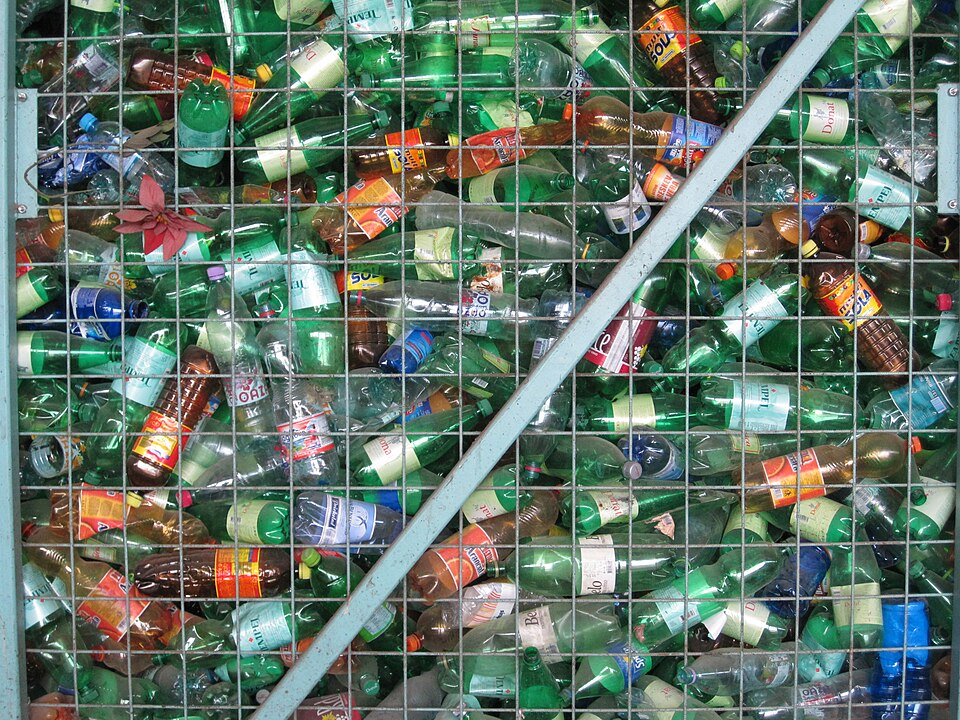
\includegraphics[width=0.49\linewidth,height=2.3cm,keepaspectratio=false]{img/bottles.jpg}\hfill
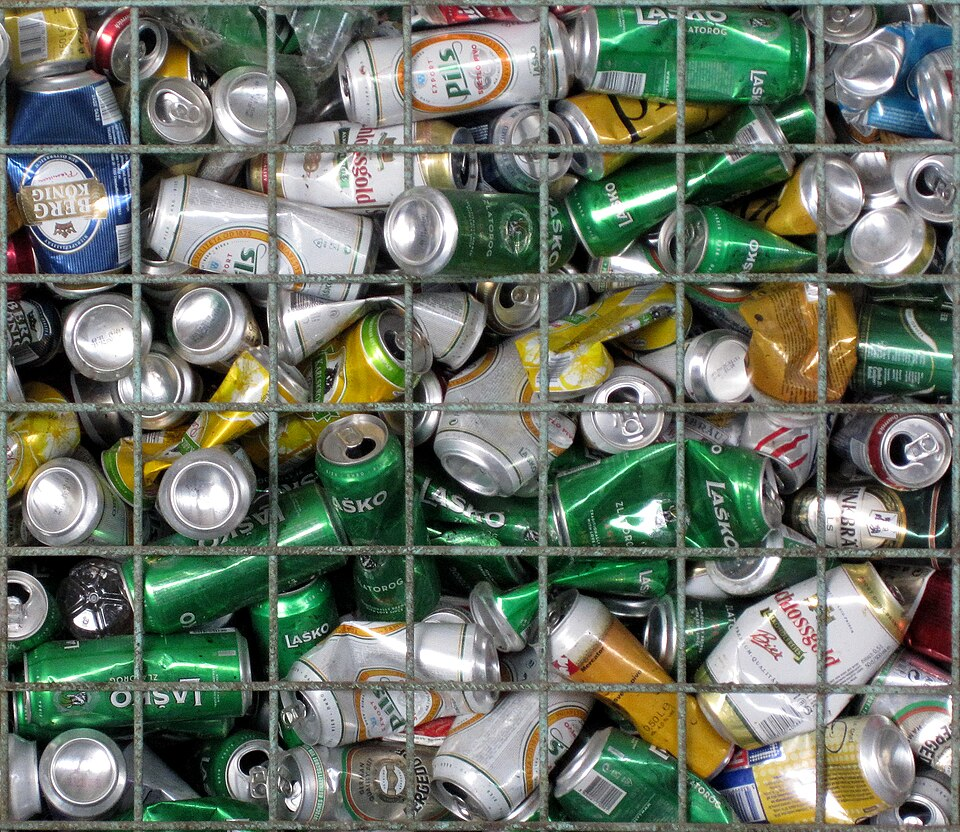
\includegraphics[width=0.49\linewidth,height=2.3cm,keepaspectratio=false]{img/cans.jpg}\par
\vskip1pt\credit{Ảnh: Wikimedia Commons -- Plastic bottles for recycling; Cans recycling (CC BY-SA 4.0)}\par\vskip6pt
\begin{tikzpicture}[font=\tiny]
  \node[bx,minimum width=1.6cm] (a) {Bỏ đúng\\vật tái chế};
  \node[bo,minimum width=1.6cm,right=0.35 of a] (b) {Nhận điểm,\\cấp độ, CO$_2$};
  \node[bg,minimum width=1.6cm,right=0.35 of b] (c) {Hình thành\\thói quen};
  \draw[ar] (a) -- (b); \draw[ar] (b) -- (c);
  \draw[ar] (c.south) -- ++(0,-0.3) -| (a.south);
\end{tikzpicture}\par
\smallnote{Vòng phản hồi: hành vi đúng $\rightarrow$ thưởng ngay $\rightarrow$ lặp lại.}
\end{columns}
\end{frame}

% ============ 4. TỔNG QUAN ============
\begin{frame}{Tổng quan hệ thống}
\footnotesize
\centering
\renewcommand{\binfs}{\fontsize{3}{3.4}\selectfont}\renewcommand{\binfss}{\fontsize{2.6}{3}\selectfont}\renewcommand{\binqrh}{0.42cm}
\begin{tikzpicture}[font=\scriptsize]
  \actor{hs}{(0,1.2)}{Học sinh};
  \begin{scope}[shift={(1.2,-0.1)},scale=0.44]\binfront\end{scope}
  \node[font=\tiny,align=center] at (2.08,-0.45) {\textbf{Thùng rác thông minh}\\AI tại chỗ, acquy + mặt trời};
  \node[bx,minimum height=1cm,text width=1.9cm] (gw) at (5.4,1.4) {\faBroadcastTower\\[1pt]\textbf{Gateway LoRa}\\ESP32 + SX127x};
  \node[bx,minimum height=1cm,text width=2.1cm] (sv) at (8.7,1.4) {\faServer\\[1pt]\textbf{Server}\\MQTT, API, CSDL};
  \node[bo,minimum height=1cm,text width=1.9cm] (app) at (12,1.4) {\faMobile*\\[1pt]\textbf{Ứng dụng}\\điểm, bản đồ};
  \node[bw,text width=2.6cm] (dash) at (8.7,-0.05) {\faChartBar~Bảng điều khiển\\nhà trường / thu gom};
  \draw[ard] (2.85,3.4) .. controls (3.6,3.4) and (3.8,1.4) .. (gw.west) node[pos=0.25,above right,lbl,text=acc] {LoRa AS923};
  \draw[ar] (gw) -- (sv) node[midway,above=1pt,lbl] {Internet};
  \draw[ar,<->] (sv) -- (app) node[midway,above=1pt,lbl] {4G};
  \draw[arg] (sv) -- (dash);
  \actor{hs2}{(13.9,1.2)}{Học sinh};
  \draw[arg] (13.6,1.4) -- (app.east);
  \draw[arg,dashed] (12,0.75) |- (3.05,-1.05) node[pos=0.75,below,lbl] {quét QR dán trên thùng + GPS};
  \draw[arg] (0.35,1.35) -- (1.4,1.9);
\end{tikzpicture}
\vskip6pt
\begin{columns}[T]
\column{0.24\textwidth}\hd{\faEye~Nhận diện tại chỗ}\scriptsize MobileNet INT8 chạy trên ESP32-S3, quyết định trước khi mở cửa.
\column{0.24\textwidth}\hd{\faBatteryHalf~Tự cấp nguồn}\scriptsize Acquy + pin mặt trời; STM32 giữ ESP32-S3 ngủ sâu.
\column{0.24\textwidth}\hd{\faWifi~Kết nối tầm xa}\scriptsize LoRa thùng $\rightarrow$ gateway; đệm dữ liệu khi mất sóng.
\column{0.24\textwidth}\hd{\faTrophy~Tạo động lực}\scriptsize Credit, cấp độ, CO$_2$ tiết kiệm, bản đồ thùng.
\end{columns}
\end{frame}

% ============ 5. USE CASE ============
\begin{frame}{Tác nhân và ca sử dụng (UML Use Case)}
\footnotesize
\begin{columns}[c]
\column{0.64\textwidth}
\centering
\begin{tikzpicture}[uc/.style={ellipse,draw=navyM,fill=navyL,font=\tiny,align=center,inner sep=0.5pt,minimum width=2.25cm,minimum height=0.55cm}]
  \draw[rulec,rounded corners=3pt,fill=white] (1.3,-0.35) rectangle (7.0,4.55);
  \node[font=\tiny\bfseries,text=navy,anchor=north east] at (6.95,4.53) {Hệ thống Smart Recycling Bin};
  \node[uc] (u1) at (2.75,3.85) {Bỏ vật tái chế};
  \node[uc] (u2) at (2.75,3.0) {Quét QR nhận điểm};
  \node[uc] (u3) at (2.75,2.15) {Xem điểm, cấp độ, CO$_2$};
  \node[uc] (u4) at (2.75,1.3) {Xem bản đồ thùng};
  \node[uc,draw=accM,fill=accL] (u5) at (5.55,3.85) {Nhận diện vật (AI)};
  \node[uc,draw=accM,fill=accL] (u6) at (5.55,3.0) {Xác thực GPS, phiên};
  \node[uc] (u7) at (5.55,2.15) {Theo dõi mức đầy, pin};
  \node[uc] (u8) at (5.55,1.3) {Nhận cảnh báo đầy};
  \node[uc] (u9) at (4.15,0.25) {Quản lý thùng, hạn mức điểm};
  \draw[navyM,dashed,-{Stealth[length=3pt]}] (u1) -- node[above,font=\fontsize{4}{4}\selectfont]{«include»} (u5);
  \draw[navyM,dashed,-{Stealth[length=3pt]}] (u2) -- node[above,font=\fontsize{4}{4}\selectfont]{«include»} (u6);
  \actor{hs}{(0.45,2.6)}{Học sinh};
  \actor{qt}{(8.0,1.3)}{Nhân viên\\thu gom};
  \actor{ad}{(8.0,3.2)}{Quản trị\\(nhà trường)};
  \foreach \u in {u1,u2,u3,u4} \draw[navy,line width=0.4pt] (0.7,2.75) -- (\u.west);
  \foreach \u in {u7,u8} \draw[navy,line width=0.4pt] (7.75,1.45) -- (\u.east);
  \draw[navy,line width=0.4pt] (7.75,3.35) -- (u7.east);
  \draw[navy,line width=0.4pt] (7.75,3.35) -- (u5.east);
  \draw[navy,line width=0.4pt] (7.75,1.45) -- (u9.east);
\end{tikzpicture}
\column{0.34\textwidth}
\hd{Yêu cầu chức năng}
\begin{itemize}\setlength\itemsep{0pt}\scriptsize
  \item Phân loại 4 lớp: chai nhựa, lon, ly nhựa, vật khác.
  \item Chỉ mở cánh lật khi vật hợp lệ.
  \item Ghi: thời gian, loại, số lượng, mức đầy, pin.
  \item Tích credit qua QR + GPS.
\end{itemize}\vskip3pt
\hd{Yêu cầu phi chức năng}
\begin{itemize}\setlength\itemsep{0pt}\scriptsize
  \item Nhận diện $\le$ \hl{1 s}, chạy hoàn toàn offline.
  \item Tự vận hành nhiều ngày không nắng.
  \item Không mất bản ghi khi mất sóng.
  \item Chống gian lận điểm.
\end{itemize}
\end{columns}
\end{frame}

% ============ 6. CƠ KHÍ ============
\begin{frame}{Thiết kế cơ khí: thân thùng 3 tầng}
\footnotesize
\begin{columns}[c]
\column{0.5\textwidth}
\centering
\renewcommand{\binfs}{\fontsize{3.4}{3.9}\selectfont}\renewcommand{\binfss}{\fontsize{3}{3.4}\selectfont}\renewcommand{\binqrh}{0.5cm}
\begin{tikzpicture}[scale=0.58]
  \binfront
  \draw[mute,{Stealth[length=3pt]}-{Stealth[length=3pt]}] (-0.45,0) -- (-0.45,7) node[midway,left,font=\tiny,text=txt] {70 cm};
  \draw[mute,{Stealth[length=3pt]}-{Stealth[length=3pt]}] (0,-0.35) -- (4,-0.35) node[midway,below,font=\tiny,text=txt] {40 cm};
  \node[font=\tiny\bfseries,text=navy] at (2,8.35) {Mặt trước};
  \begin{scope}[xshift=5.6cm]
    \binsection
    \node[font=\tiny\bfseries,text=navy] at (2,8.35) {Mặt cắt};
    \draw[decorate,decoration={brace,amplitude=3pt},navyM] (4.15,6.8) -- (4.15,5.0) node[midway,right=2pt,font=\tiny,text=txt,align=left] {T1};
    \draw[decorate,decoration={brace,amplitude=3pt},navyM] (4.15,4.95) -- (4.15,4.2) node[midway,right=2pt,font=\tiny,text=txt] {T2};
    \draw[decorate,decoration={brace,amplitude=3pt},navyM] (4.15,4.1) -- (4.15,0.1) node[midway,right=2pt,font=\tiny,text=txt] {T3};
  \end{scope}
\end{tikzpicture}
\column{0.48\textwidth}
\hd{Vỏ}
Tấm \kw{fomex 5--10 mm} lắp ghép, kích thước \kw{40 $\times$ 40 $\times$ 70 cm}; nóc gắn pin mặt trời, anten LoRa.\par\vskip3pt
\hd{T1 -- Khu nhận diện (phía trước)}
Buồng có \kw{chụp che}, \kw{nền trắng}, \kw{đèn LED} chiếu đều: ảnh ổn định, không phụ thuộc ánh sáng ngoài. Camera đặt trên đỉnh nhìn xuống.\par\vskip3pt
\hd{T2 -- Cánh lật servo}
Đáy buồng là cánh lật: \hl{nằm ngang (đóng)} khi chưa xác nhận; lật \kw{trái} $\rightarrow$ khoang nhựa, lật \kw{phải} $\rightarrow$ khoang lon.\par\vskip3pt
\hd{T3 -- Khoang chứa}
Vách ngăn chia 2 khoang, mỗi khoang có \kw{cảm biến siêu âm} đo mức đầy; đáy đặt acquy và mạch (hạ trọng tâm).
\end{columns}
\end{frame}

% ============ 7. SƠ ĐỒ KHỐI ============
\begin{frame}{Kiến trúc phần cứng (sơ đồ khối)}
\centering
\begin{tikzpicture}[
  m/.style={bx,text width=2.35cm,minimum height=0.62cm,font=\tiny},
  io/.style={lbl,fill=white,font=\fontsize{4.5}{5}\selectfont,text=mute}]
  \node[draw=navy,fill=navy,text=white,rounded corners=2pt,align=center,text width=2.9cm,minimum height=3.3cm,font=\scriptsize] (esp) at (7,4.15)
    {\textbf{ESP32-S3}\\[1pt]{\tiny N16R8 -- 8 MB PSRAM}\\[3pt]{\tiny TFLite Micro + ESP-NN\\FreeRTOS\\điều phối phiên làm việc}};
  % trái
  \node[m] (cam) at (2.0,5.5) {\faCamera~Camera OV2640};
  \node[m] (led) at (2.0,4.6) {\faLightbulb~Đèn LED trắng};
  \node[m] (us)  at (2.0,3.7) {\faRulerVertical~Siêu âm $\times$2 (mức đầy)};
  \node[m] (rtc) at (2.0,2.8) {\faClock~RTC DS3231};
  \node[m,draw=accM,fill=accL] (pir) at (2.0,1.6) {\faWalking~Cảm biến tiệm cận};
  % phải
  \node[m] (tft) at (12.0,5.5) {\faDesktop~TFT 2.8'' ILI9341};
  \node[m] (sv)  at (12.0,4.6) {\faCog~Servo cánh lật};
  \node[m,draw=accM,fill=accL] (lora) at (12.0,3.7) {\faBroadcastTower~LoRa SX1276 (AS923)};
  \node[m,dashed] (buf) at (12.0,2.8) {\faDatabase~Bộ đệm bản ghi (flash)};
  \node[m,draw=grn,fill=grnL] (sw) at (12.0,1.6) {\faToggleOn~Khóa tải (MOSFET)};
  % STM32
  \node[bo,text width=2.9cm,minimum height=0.75cm,font=\tiny] (stm) at (7,1.6) {\textbf{STM32L0} -- gác cổng năng lượng\\Stop mode, đo áp acquy};
  % nguồn
  \node[bg,font=\tiny] (pv) at (1.4,0.2) {\faSun~Pin mặt trời 20 W};
  \node[bg,font=\tiny] (chg) at (4.4,0.2) {Bộ sạc MPPT};
  \node[bg,font=\tiny] (bat) at (7,0.2) {\faCarBattery~Acquy 12 V 7 Ah};
  \node[bg,font=\tiny] (bk) at (9.8,0.2) {Buck 5 V / LDO 3,3 V};
  \draw[grn,-{Stealth[length=3pt]},line width=0.7pt] (pv) -- (chg); \draw[grn,-{Stealth[length=3pt]},line width=0.7pt] (chg) -- (bat);
  \draw[grn,-{Stealth[length=3pt]},line width=0.7pt] (bat) -- (bk); \draw[grn,-{Stealth[length=3pt]},line width=0.7pt] (bk) -| (sw);
  \draw[grn,-{Stealth[length=3pt]},line width=0.7pt] (bat) -- (stm);
  \draw[grn,-{Stealth[length=3pt]},line width=0.7pt] (sw.north) -- ++(0,0.3) -| ($(esp.south east)+(-0.3,0)$) node[pos=0.3,above,io]{nguồn 5 V};
  % kết nối
  \draw[ar] (cam) -- (esp.west |- cam) node[midway,io]{DVP};
  \draw[ar] (esp.west |- led) -- (led) node[midway,io]{GPIO};
  \draw[ar] (us) -- (esp.west |- us) node[midway,io]{GPIO};
  \draw[ar,<->] (rtc) -- (esp.west |- rtc) node[midway,io]{I²C};
  \draw[ar] (esp.east |- tft) -- (tft) node[midway,io]{SPI};
  \draw[ar] (esp.east |- sv) -- (sv) node[midway,io]{PWM};
  \draw[ar,<->] (esp.east |- lora) -- (lora) node[midway,io]{SPI};
  \draw[ar,<->] (esp.east |- buf) -- (buf) node[midway,io]{LittleFS};
  \draw[ard] (pir) -- (stm) node[midway,above,io,text=acc]{ngắt đánh thức};
  \draw[ard] (stm) -- (sw) node[midway,above,io,text=acc]{bật/tắt};
  \draw[ard] ($(stm.north)+(-0.6,0)$) -- ($(esp.south)+(-0.6,0)$) node[midway,left,io,text=acc]{UART};
\end{tikzpicture}
\vskip2pt
{\scriptsize\kw{Nguyên tắc:} chỉ STM32 (vài µA) luôn thức; ESP32-S3, camera, TFT, servo \hl{bị ngắt nguồn} cho tới khi có người đến.\par}
\end{frame}

% ============ 8. LINH KIỆN ============
\begin{frame}{Linh kiện chính}
\centering
\begin{minipage}{0.235\textwidth}\centering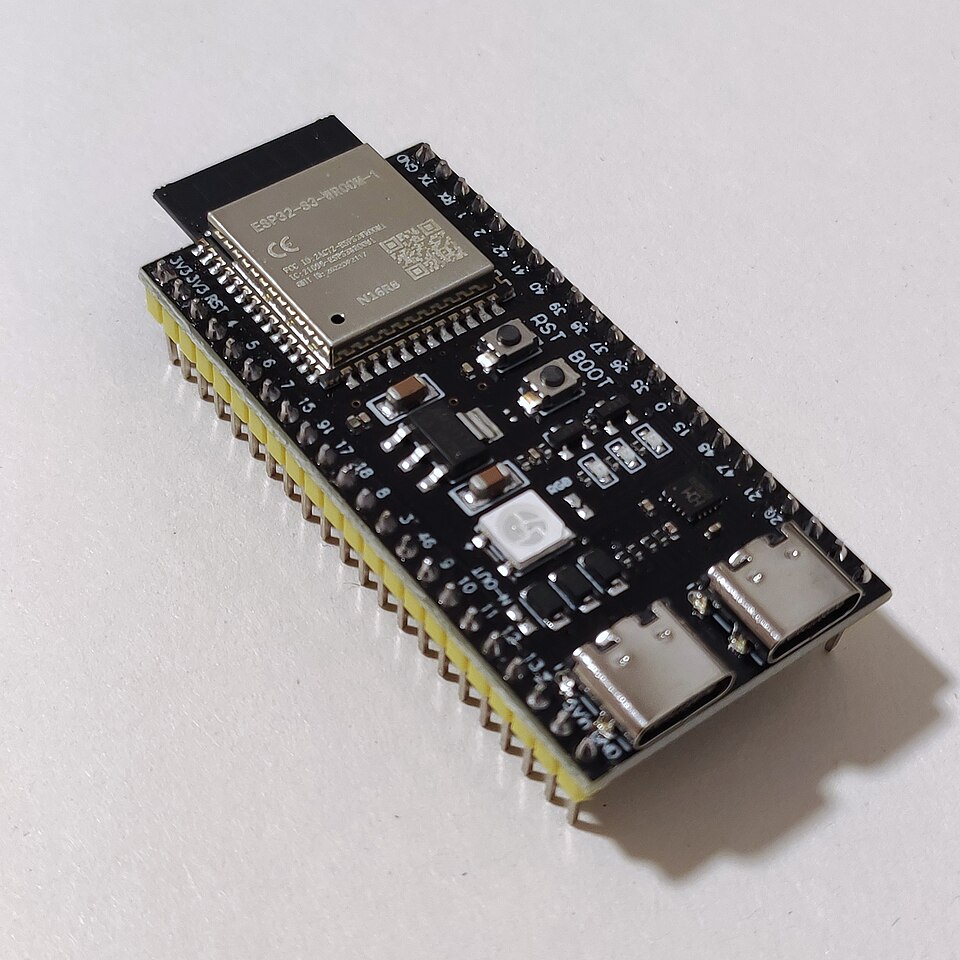
\includegraphics[height=1.55cm]{img/esp32s3.jpg}\\{\tiny ESP32-S3 DevKit}\end{minipage}\hfill
\begin{minipage}{0.235\textwidth}\centering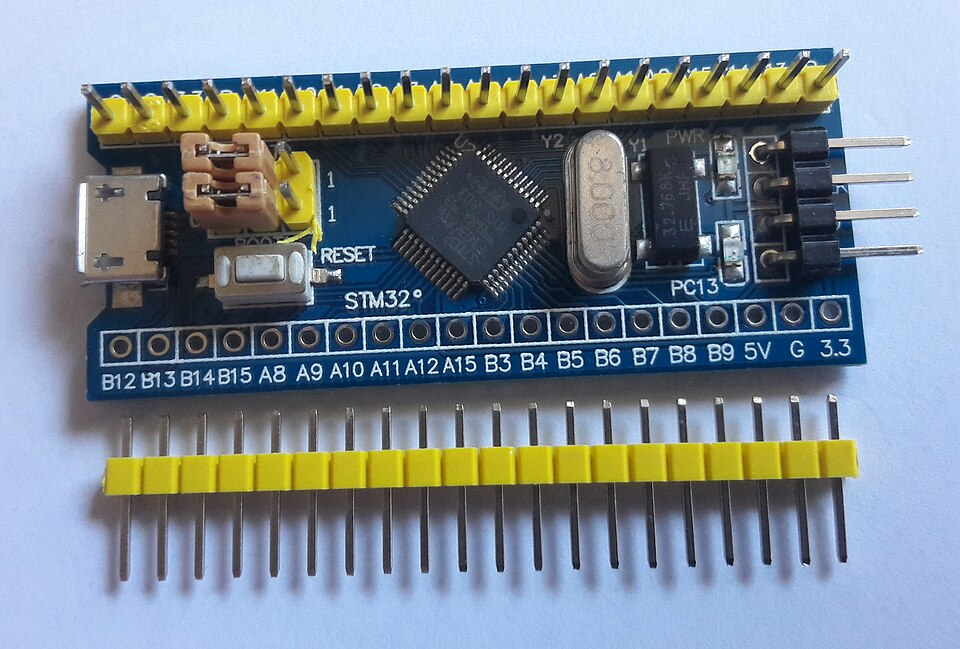
\includegraphics[height=1.55cm]{img/stm32.jpg}\\{\tiny STM32 (bo phát triển)}\end{minipage}\hfill
\begin{minipage}{0.235\textwidth}\centering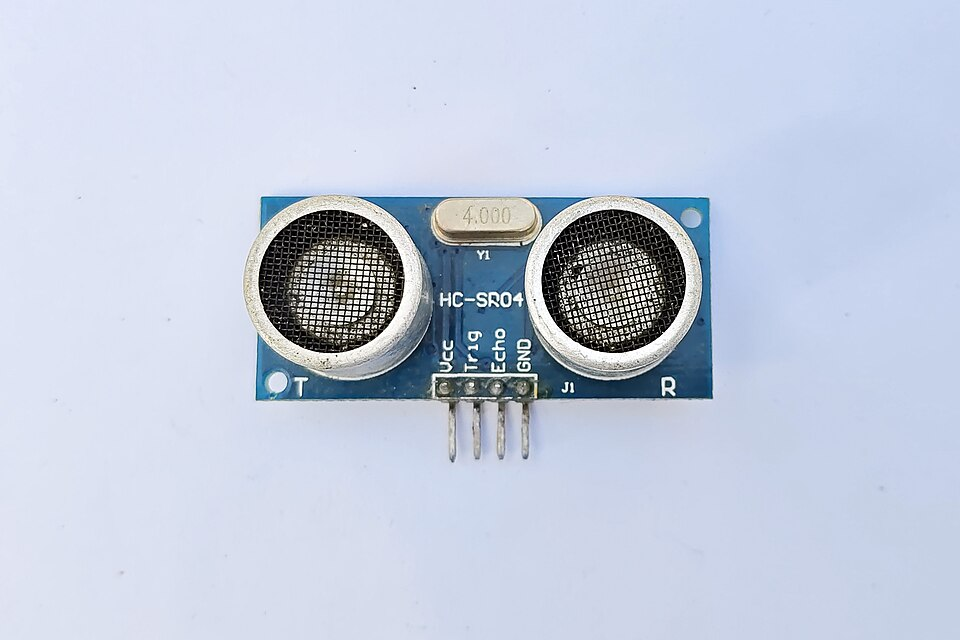
\includegraphics[height=1.55cm]{img/hcsr04.jpg}\\{\tiny Cảm biến siêu âm HC-SR04}\end{minipage}\hfill
\begin{minipage}{0.235\textwidth}\centering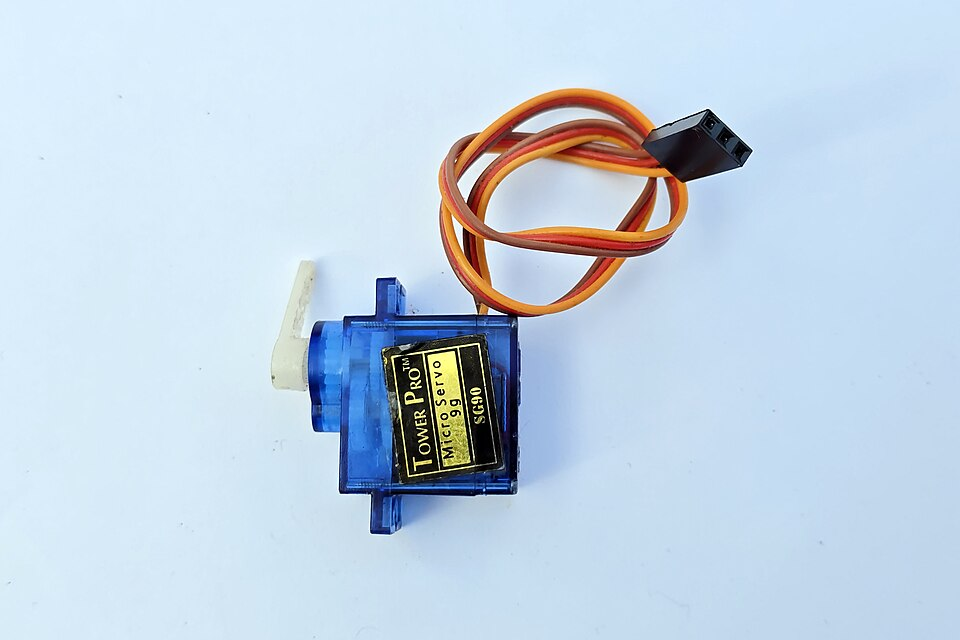
\includegraphics[height=1.55cm]{img/sg90.jpg}\\{\tiny Servo (minh họa)}\end{minipage}\par
\vskip1pt\credit{Ảnh: Wikimedia Commons -- ESP32-S3 on paper, Core Learning Board STM32F103, HC SR04 Ultrasonic Module (CC BY-SA 4.0); Tower Pro SG90 (CC BY-SA 4.0).}\par
\vskip3pt
\scriptsize
\renewcommand{\arraystretch}{1.05}
\begin{tabularx}{\linewidth}{@{}>{\bfseries\color{navy}}l l l X@{}}
\toprule
\textbf{Khối} & \textbf{Linh kiện đề xuất} & \textbf{Giao tiếp} & \textbf{Vai trò}\\\midrule
Xử lý chính & ESP32-S3 N16R8 + camera OV2640 & DVP & Chụp ảnh, chạy AI, điều phối, giao diện\\
Gác cổng & STM32L0 (hoặc STM32WL ở bản mở rộng) & GPIO, UART & Ngủ sâu, đánh thức, giám sát pin\\
Hiển thị & TFT 2.8'' ILI9341, 320$\times$240 & SPI & Kết quả, trạng thái thùng, thông tin môi trường\\
Cơ cấu & Servo MG996R (mô-men lớn) & PWM & Lật cánh trái / phải\\
Cảm biến & HC-SR04 $\times$2; cảm biến tiệm cận PIR/IR & GPIO & Đo mức đầy; đánh thức hệ thống\\
Thời gian & RTC DS3231 & I²C & Dấu thời gian chính xác khi offline\\
Truyền thông & LoRa SX1276/SX1262, AS923 & SPI & Gửi bản ghi về gateway\\
Nguồn & Acquy 12 V 7 Ah, pin MT 20 W, sạc MPPT, buck & -- & Cấp nguồn tự chủ\\
\bottomrule
\end{tabularx}
\end{frame}

% ============ 9. NĂNG LƯỢNG ============
\begin{frame}{Quản lý năng lượng}
\footnotesize
\begin{columns}[T]
\column{0.47\textwidth}
\hd{Các chế độ hoạt động}
\centering
\begin{tikzpicture}[s/.style={bx,text width=1.7cm,minimum height=0.85cm,font=\tiny}]
  \node[s,draw=grn,fill=grnL] (sl) at (0,0) {\textbf{Ngủ}\\STM32 Stop\\cảm biến tiệm cận};
  \node[s,draw=accM,fill=accL] (ac) at (3.6,0) {\textbf{Phiên làm việc}\\ESP32-S3, camera,\\TFT, LED};
  \node[s] (hb) at (1.8,-1.75) {\textbf{Báo cáo định kỳ}\\đo đầy + LoRa};
  \draw[ar] (sl.north) to[bend left=25] node[above,lbl]{có người đến} (ac.north);
  \draw[ar] (ac.south west) to[bend left=15] node[below,lbl,pos=0.4]{hết 30 s không dùng} (sl.south east);
  \draw[arg] (sl.south) |- node[pos=0.3,left,lbl]{30 phút} (hb.west);
  \draw[arg] (hb.east) -| (ac.south) node[pos=0.25,below,lbl]{} ;
  \node[lbl,text=mute,align=left] at (4.45,-1.45) {đánh thức\\ESP32 nếu cần};
\end{tikzpicture}\par\vskip3pt
\raggedright
\hd{Chuỗi nguồn}
Pin mặt trời $\rightarrow$ sạc MPPT $\rightarrow$ acquy 12 V $\rightarrow$ buck 5 V. STM32 đo áp acquy, báo pin yếu qua LoRa và
\hl{từ chối mở phiên} khi áp quá thấp để bảo vệ acquy.
\column{0.51\textwidth}
\hd{Ngân sách năng lượng (ước tính sơ bộ)}
\scriptsize
\begin{tabularx}{\linewidth}{@{}X r r@{}}
\toprule
\textbf{Trạng thái} & \textbf{Công suất} & \textbf{Thời gian/ngày}\\\midrule
Ngủ (STM32 + PIR) & $\approx$ 10 mW & 24 h\\
Phiên (ESP32-S3 + cam + TFT + LED) & $\approx$ 2,5 W & 200 lượt $\times$ 10 s\\
Servo lật & $\approx$ 3 W & 200 $\times$ 1 s\\
LoRa phát (SF7--SF9) & $\approx$ 0,4 W & $<$ 1 phút\\\midrule
\textbf{Tổng (kể cả hao hụt 30\%)} & & \textbf{$\approx$ 2,5 Wh}\\
\bottomrule
\end{tabularx}\vskip4pt
\begin{itemize}\setlength\itemsep{1pt}
  \item Acquy 12 V 7 Ah $\approx$ \kw{84 Wh} (dùng 50\% $\approx$ 42 Wh) $\Rightarrow$ \hl{$\approx$ 2 tuần} không nắng.
  \item Pin MT 20 W, 3--4 giờ nắng hiệu dụng $\approx$ 60 Wh/ngày: dư nhiều lần nhu cầu.
\end{itemize}
\smallnote{Số liệu là ước tính thiết kế; sẽ đo dòng thực tế từng chế độ để hiệu chỉnh.}
\end{columns}
\end{frame}

% ============ 10. PIPELINE AI ============
\begin{frame}{Nhận diện AI trên thiết bị: pipeline}
\centering
\begin{tikzpicture}[p/.style={bx,text width=1.75cm,minimum height=1.05cm,font=\tiny}]
  \node[p] (a) at (0,0) {\faCamera\\\textbf{Chụp ảnh}\\320$\times$240, LED bật};
  \node[p] (b) at (2.45,0) {\faCrop\\\textbf{Tiền xử lý}\\cắt vùng nền trắng, 96$\times$96};
  \node[p,draw=accM,fill=accL] (c) at (4.9,0) {\faBrain\\\textbf{MobileNetV2}\\$\alpha$=0.35, INT8\\TFLite Micro};
  \node[p] (d) at (7.35,0) {\faChartBar\\\textbf{Softmax}\\4 lớp};
  \node[p,draw=grn,fill=grnL] (e) at (9.8,0) {\faCheckDouble\\\textbf{Quyết định}\\ngưỡng + bỏ phiếu};
  \foreach \x/\y in {a/b,b/c,c/d,d/e} \draw[ar] (\x) -- (\y);
  \node[bg,text width=1.6cm,font=\tiny] (ok) at (12.4,0.55) {Hợp lệ $\rightarrow$\\lật cánh};
  \node[bo,text width=1.6cm,font=\tiny] (no) at (12.4,-0.55) {Từ chối $\rightarrow$\\báo trên TFT};
  \draw[ar] (e) -- (ok.west); \draw[ard] (e) -- (no.west);
\end{tikzpicture}
\vskip8pt
\footnotesize
\begin{columns}[T]
\column{0.33\textwidth}
\hd{Mô hình}
\begin{itemize}\setlength\itemsep{1pt}\scriptsize
  \item MobileNetV2 (depthwise separable conv): ít tham số, hợp vi điều khiển.
  \item Lượng tử INT8: mô hình \kw{$<$ 1 MB}, nằm trong flash/PSRAM.
  \item ESP-NN tăng tốc phép tích chập trên S3.
\end{itemize}
\column{0.30\textwidth}
\hd{Luật quyết định}
\scriptsize
Chấp nhận khi $p_{\max} \ge \tau$ ($\tau \approx 0{,}8$) và \kw{cùng nhãn ở 2/3 khung} liên tiếp.
Ngược lại: yêu cầu đặt lại; \hl{lớp ``vật khác'' luôn bị từ chối}.
\column{0.33\textwidth}
\hd{Ví dụ đầu ra}
\begin{tikzpicture}[font=\tiny]
  \foreach \n/\v/\c [count=\i] in {Chai nhựa/0.91/grn,Lon/0.04/navyM,Ly nhựa/0.03/navyM,Vật khác/0.02/navyM}{
    \node[anchor=east] at (0,-\i*0.28) {\n};
    \fill[\c] (0.05,-\i*0.28-0.09) rectangle ++(\v*2.6,0.18);
    \node[anchor=west] at (\v*2.6+0.08,-\i*0.28) {\v};}
  \draw[acc,dashed] (0.05+0.8*2.6,-0.1) -- ++(0,-1.1) node[below,text=acc]{$\tau$};
\end{tikzpicture}
\end{columns}
\vskip8pt
\begin{tikzpicture}\node[bo,text width=0.95\linewidth,align=left,font=\scriptsize,inner sep=5pt]{\textbf{\textcolor{acc}{Vì sao chạy AI ngay trên thùng (edge AI)?}}\quad
LoRa chỉ gửi được vài chục byte mỗi gói nên \kw{không thể gửi ảnh} về server; xử lý tại chỗ cho phản hồi tức thì,
hoạt động khi mất mạng và \kw{không lưu/truyền ảnh} học sinh.};\end{tikzpicture}
\end{frame}

% ============ 11. DỮ LIỆU & HUẤN LUYỆN ============
\begin{frame}{Dữ liệu và huấn luyện mô hình}
\footnotesize
\begin{columns}[T]
\column{0.5\textwidth}
\hd{Tập dữ liệu (tự thu thập trong buồng nhận diện)}
\scriptsize
\begin{tabularx}{\linewidth}{@{}>{\bfseries}l X r@{}}
\toprule
\textbf{Lớp} & \textbf{Ví dụ} & \textbf{Mục tiêu}\\\midrule
Chai nhựa & PET 330 ml -- 1,5 l, có/không nhãn, móp & $\ge$ 500 ảnh\\
Lon & nhôm 250--330 ml, móp, nhiều màu & $\ge$ 500 ảnh\\
Ly nhựa & ly trà sữa, ly cà phê, có/không nắp & $\ge$ 500 ảnh\\
Vật khác & tay, giấy, hộp sữa, vỏ bánh, chai thủy tinh & $\ge$ 800 ảnh\\
\bottomrule
\end{tabularx}\vskip3pt
\begin{itemize}\setlength\itemsep{1pt}
  \item Chụp bằng \kw{chính camera và đèn của thùng} để tránh lệch miền dữ liệu.
  \item Tăng cường: xoay, lật, độ sáng, che khuất một phần.
  \item Chia train/val/test theo \hl{vật thể}, không theo ảnh, tránh rò rỉ.
\end{itemize}
\column{0.48\textwidth}
\hd{Quy trình}
\centering
\begin{tikzpicture}[q/.style={bx,text width=3.9cm,font=\tiny,minimum height=0.5cm}]
  \node[q] (1) at (0,0) {Học chuyển giao từ trọng số ImageNet};
  \node[q] (2) at (0,-0.72) {Tinh chỉnh toàn mạng (Keras)};
  \node[q,draw=accM,fill=accL] (3) at (0,-1.44) {Lượng tử INT8 (PTQ, có tập hiệu chỉnh)};
  \node[q] (4) at (0,-2.16) {Xuất .tflite $\rightarrow$ mảng C};
  \node[q,draw=grn,fill=grnL] (5) at (0,-2.88) {Nạp lên ESP32-S3, đo trên thiết bị};
  \foreach \i/\j in {1/2,2/3,3/4,4/5} \draw[ar] (\i) -- (\j);
\end{tikzpicture}\par\vskip4pt
\raggedright
\hd{Chỉ tiêu cần đạt}
\scriptsize
Độ chính xác test \kw{$\ge$ 90\%}; nhận nhầm ``vật khác'' thành hợp lệ \hl{$\le$ 3\%} (quan trọng hơn độ chính xác chung); thời gian suy luận \kw{$\le$ 500 ms}.
\end{columns}
\end{frame}

% ============ 12. MÁY TRẠNG THÁI ============
\begin{frame}{Phần mềm thiết bị: máy trạng thái (UML State Machine)}
\centering
\begin{tikzpicture}[st/.style={bx,rounded corners=5pt,text width=1.95cm,minimum height=0.78cm,font=\tiny},
  t/.style={lbl,font=\fontsize{4.8}{5.5}\selectfont,align=center}]
  \fill[navy] (-1.35,3.55) circle (0.1);
  \node[st,draw=grn,fill=grnL] (sl) at (0.4,3.55) {\textbf{Ngủ sâu}\\ESP32 tắt nguồn};
  \node[st] (w) at (4.2,3.55) {\textbf{Chờ vật}\\TFT: hướng dẫn, tin môi trường};
  \node[st,draw=accM,fill=accL] (r) at (8.0,3.55) {\textbf{Nhận diện}\\chụp + suy luận};
  \node[st] (o) at (11.8,3.55) {\textbf{Lật cánh}\\trái / phải};
  \node[st,draw=red!70,fill=red!5] (rj) at (8.0,5.15) {\textbf{Từ chối}\\TFT: ``vật không hợp lệ''};
  \node[st] (hb) at (0.4,1.85) {\textbf{Báo cáo định kỳ}\\đo đầy, gửi LoRa};
  \node[st] (lg) at (11.8,1.85) {\textbf{Ghi nhận}\\lưu đệm + gửi LoRa};
  \node[st,draw=red!70,fill=red!5] (fl) at (11.8,0.35) {\textbf{Khóa}\\báo đầy, chờ thu gom};
  \draw[ar] (-1.25,3.55) -- (sl);
  \draw[ar] (sl) -- node[t,above]{tiệm cận:\\có người} (w);
  \draw[ar] (w) -- node[t,above]{nền thay đổi:\\có vật} (r);
  \draw[ar] (r) -- node[t,above]{[hợp lệ]} (o);
  \draw[ar] (o) -- node[t,right]{cánh đóng,\\buồng trống} (lg);
  \draw[ar] (r) -- node[t,right]{[vật khác /\\không chắc]} (rj);
  \draw[ar] (rj.west) -| node[t,pos=0.3,above]{lấy vật ra} ($(w.north)+(0.4,0)$);
  \draw[ar] ($(w.north)+(-0.4,0)$) |- ($(sl.north)+(0,0.85)$) node[t,pos=0.75,above]{30 s không ai dùng} -- (sl.north);
  \draw[ar] (lg.west) -| node[t,pos=0.25,above]{[chưa đầy]} (w.south);
  \draw[ar] (lg) -- node[t,right]{[mức đầy $\ge$ 90\%]} (fl);
  \draw[ar] (fl.west) -| node[t,pos=0.3,above]{đã thu gom} (hb.south);
  \draw[ar] ($(sl.south)+(-0.35,0)$) -- node[t,left]{hẹn giờ\\30 phút} ($(hb.north)+(-0.35,0)$);
  \draw[ar] ($(hb.north)+(0.35,0)$) -- node[t,right]{xong} ($(sl.south)+(0.35,0)$);
\end{tikzpicture}
\vskip4pt
{\scriptsize\kw{Kiểm tra sau khi lật:} chụp lại buồng, phải \hl{trống} mới ghi nhận -- chặn trò kéo vật bằng dây để bỏ nhiều lần.\par}
\end{frame}

% ============ 13. SEQUENCE ============
\begin{frame}{Luồng bỏ rác và nhận điểm (UML Sequence)}
\centering
\begin{tikzpicture}[m/.style={-{Stealth[length=3.5pt]},navy,line width=0.5pt},r/.style={m,dashed,navyM},
  t/.style={font=\fontsize{4.8}{5.5}\selectfont,above,inner sep=1pt},
  sl/.style={font=\fontsize{4.8}{5.5}\selectfont,right,align=left,inner sep=1pt}]
  \foreach \x/\n/\s in {0.6/Học sinh/bw,3.2/Ứng dụng/bo,6.0/Thùng (ESP32-S3)/bx,8.7/Gateway LoRa/bx,11.4/Server/bg}{
    \node[\s,text width=1.75cm,font=\tiny\bfseries] at (\x,5.6) {\n};
    \draw[rulec,dashed] (\x,5.35) -- (\x,0.45);}
  \fill[accL,draw=accM] (11.32,4.6) rectangle (11.48,3.75);
  \fill[navyL,draw=navyM] (5.92,3.4) rectangle (6.08,2.45);
  \fill[grnL,draw=grn] (11.32,1.6) rectangle (11.48,0.75);
  \draw[m] (0.6,5.0) -- node[t]{1. quét QR dán trên thùng} (3.2,5.0);
  \draw[m] (3.2,4.6) -- node[t]{2. bin\_id, GPS, token người dùng (4G/HTTPS)} (11.32,4.6);
  \draw[m] (11.48,4.4) -- ++(0.35,0) |- (11.48,4.1) node[sl,pos=0.25,xshift=0.35cm]{3. GPS trong bán kính?\\mở phiên 60 s};
  \draw[r] (11.32,3.8) -- node[t]{4. ``phiên đã mở''} (3.2,3.8);
  \draw[m] (0.6,3.4) -- node[t]{5. đưa vật vào buồng} (5.92,3.4);
  \draw[m] (6.08,3.2) -- ++(0.35,0) |- (6.08,2.9) node[sl,pos=0.25,xshift=0.35cm]{6. AI: hợp lệ, lật cánh};
  \draw[r] (5.92,2.6) -- node[t]{7. TFT: kết quả + thông tin môi trường} (0.6,2.6);
  \draw[m] (6.08,2.3) -- node[t]{8. bản ghi \{t, loại, đầy, pin\} (LoRa)} (8.7,2.3);
  \draw[r] (8.7,1.95) -- node[t]{9. ACK} (6.08,1.95);
  \draw[m] (8.7,1.6) -- node[t]{10. chuyển tiếp (MQTT)} (11.32,1.6);
  \draw[m] (11.48,1.4) -- ++(0.35,0) |- (11.48,1.1) node[sl,pos=0.25,xshift=0.35cm]{11. gán vào phiên,\\kiểm hạn mức, +credit};
  \draw[r] (11.32,0.8) -- node[t]{12. +credit, CO$_2$, cấp độ (thông báo đẩy)} (3.2,0.8);
\end{tikzpicture}
\vskip2pt
{\scriptsize Không có ACK ở bước 9 $\Rightarrow$ bản ghi nằm trong bộ đệm flash, gửi lại ở lần kế tiếp; dấu thời gian từ RTC nên server vẫn ghép đúng phiên.\par}
\end{frame}

% ============ 14. LORA ============
\begin{frame}{Truyền thông LoRa và gói tin}
\footnotesize
\begin{columns}[T]
\column{0.46\textwidth}
\hd{Cấu hình liên kết}
\begin{itemize}\setlength\itemsep{1pt}\scriptsize
  \item Băng tần \kw{AS923} (dải 920--923 MHz dùng tại Việt Nam).
  \item BW 125 kHz, \kw{SF7--SF9} tùy khoảng cách; phát $\le$ 14 dBm.
  \item Gói $\approx$ 14 byte $\Rightarrow$ thời gian phát $\approx$ 50--200 ms.
  \item Tuân thủ giới hạn thời gian chiếm kênh: gộp bản ghi, không phát liên tục.
\end{itemize}\vskip3pt
\hd{Lưu đệm khi mất sóng}
\scriptsize
Bản ghi được ghi vào \kw{bộ đệm vòng trên flash} trước khi phát; chỉ xóa khi gateway \kw{ACK}. Mất sóng $\Rightarrow$ gửi gộp khi có lại.
Dấu thời gian lấy từ \kw{RTC DS3231}, không phụ thuộc mạng.\par\vskip4pt
\centering
\begin{tikzpicture}[font=\tiny]
  \node[bx] (b1) at (0,0.5) {Thùng 1}; \node[bx] (b2) at (0,-0.1) {Thùng 2}; \node[bx] (b3) at (0,-0.7) {Thùng n};
  \node[bo,text width=1.3cm] (g) at (2.4,-0.1) {Gateway\\LoRa};
  \node[bg,text width=1.2cm] (s) at (4.6,-0.1) {Server\\MQTT};
  \foreach \b in {b1,b2,b3} \draw[ard] (\b) -- (g);
  \draw[ar] (g) -- node[above,lbl]{Wi-Fi/4G} (s);
\end{tikzpicture}
\column{0.52\textwidth}
\hd{Định dạng gói uplink (14 byte)}
\scriptsize
\begin{tabularx}{\linewidth}{@{}l c X@{}}
\toprule
\textbf{Trường} & \textbf{Byte} & \textbf{Ý nghĩa}\\\midrule
\texttt{bin\_id} & 2 & mã thùng\\
\texttt{seq} & 2 & số thứ tự, chống trùng/mất gói\\
\texttt{ts} & 4 & thời gian Unix (RTC)\\
\texttt{type} & 1 & 0 chai nhựa, 1 lon, 2 ly nhựa, 3 từ chối, 0xF báo cáo định kỳ\\
\texttt{count} & 1 & số vật trong bản ghi\\
\texttt{fill} & 2 & mức đầy khoang nhựa / lon (\%)\\
\texttt{batt} & 1 & mức pin (\%)\\
\texttt{flags} & 1 & đầy, pin yếu, lỗi cảm biến, cửa kẹt\\
\bottomrule
\end{tabularx}\vskip3pt
\smallnote{Gói kèm mã xác thực (MIC/HMAC) để server loại bỏ bản ghi giả mạo.}
\end{columns}
\end{frame}

% ============ 15. SERVER & CSDL ============
\begin{frame}{Server và cơ sở dữ liệu}
\footnotesize
\begin{columns}[T]
\column{0.36\textwidth}
\hd{Kiến trúc backend}
\centering
\begin{tikzpicture}[k/.style={bx,text width=3.3cm,font=\tiny,minimum height=0.48cm}]
  \node[k,draw=accM,fill=accL] (g) at (0,0) {Gateway LoRa};
  \node[k] (mq) at (0,-0.75) {MQTT broker (Mosquitto)};
  \node[k] (be) at (0,-1.5) {Dịch vụ backend (FastAPI)\\giải mã, xác thực, tính điểm};
  \node[bg,text width=1.0cm,font=\tiny] (db) at (0,-2.75) {\faDatabase\\PostgreSQL};
  \node[bw,text width=1.0cm,font=\tiny] (ap) at (-1.3,-2.75) {\faMobile*\\App (REST)};
  \node[bw,text width=1.0cm,font=\tiny] (da) at (1.3,-2.75) {\faDesktop\\Web quản trị};
  \draw[ar] (g) -- (mq); \draw[ar] (mq) -- (be); \draw[ar,<->] (be) -- (db);
  \draw[ar,<->] ($(be.south)+(-1.2,0)$) -- (ap.north); \draw[ar,<->] ($(be.south)+(1.2,0)$) -- (da.north);
\end{tikzpicture}\par\vskip3pt\raggedright
\scriptsize Web quản trị: bản đồ thùng, mức đầy, pin, \hl{cảnh báo cần thu gom}, thống kê theo lớp/khối.
\column{0.62\textwidth}
\hd{Lược đồ dữ liệu (ER)}
\centering
\begin{tikzpicture}[e/.style={draw=navyM,rectangle split,rectangle split parts=2,rectangle split part fill={navy,white},inner sep=2pt,font=\fontsize{5.2}{6}\selectfont,align=left},
  c/.style={font=\fontsize{5}{5}\selectfont,text=navyM}]
  \node[e,anchor=north] (u) at (0,0) {\textcolor{white}{\bfseries users}\nodepart{two}\begin{tabular}{@{}l@{}}\underline{id}\\ho\_ten, lop\\credit, cap\_do\\co2\_g\end{tabular}};
  \node[e,anchor=north] (s) at (2.75,0) {\textcolor{white}{\bfseries sessions}\nodepart{two}\begin{tabular}{@{}l@{}}\underline{id}\\user\_id, bin\_id\\gps, do\_chinh\_xac\\bat\_dau, het\_han\end{tabular}};
  \node[e,anchor=north] (b) at (5.6,0) {\textcolor{white}{\bfseries bins}\nodepart{two}\begin{tabular}{@{}l@{}}\underline{id}\\vi\_do, kinh\_do\\fill\_nhua, fill\_lon\\pin, last\_seen\end{tabular}};
  \node[e,anchor=north] (c) at (0.4,-2.0) {\textcolor{white}{\bfseries credit\_logs}\nodepart{two}\begin{tabular}{@{}l@{}}\underline{id}\\user\_id, deposit\_id\\diem, co2\_g, ngay\end{tabular}};
  \node[e,anchor=north] (d) at (4.4,-2.0) {\textcolor{white}{\bfseries deposits}\nodepart{two}\begin{tabular}{@{}l@{}}\underline{id}\\bin\_id, seq, ts\\loai, so\_luong\\session\_id\end{tabular}};
  \draw[navyM] (u) -- node[c,above,pos=0.15]{1} node[c,above,pos=0.85]{*} (s);
  \draw[navyM] (s) -- node[c,above,pos=0.15]{*} node[c,above,pos=0.85]{1} (b);
  \draw[navyM] (b.south) |- node[c,right,pos=0.1]{1} node[c,above,pos=0.9]{*} (d.east);
  \draw[navyM] (s.south) -- ++(0,-0.75) node[c,right,pos=0.3]{1} -| node[c,right,pos=0.8]{*} ($(d.north)+(-0.3,0)$);
  \draw[navyM] (u.south -| c.north) -- node[c,left,pos=0.15]{1} node[c,left,pos=0.85]{*} (c.north);
  \draw[navyM] (d.west) -- node[c,above,pos=0.15]{1} node[c,above,pos=0.85]{1} (c.east |- d.west);
\end{tikzpicture}\par\vskip2pt\raggedright
\scriptsize Ràng buộc \texttt{UNIQUE(bin\_id, seq)} trên \texttt{deposits}: gói LoRa gửi lại không bị cộng điểm hai lần.
\end{columns}
\end{frame}

% ============ 16. APP ============
\begin{frame}{Ứng dụng di động}
\centering
\begin{tikzpicture}
  \phone{0}{Quét QR}{
    \draw[acc,line width=0.8pt] (0.45,1.7) -- (0.45,1.55) -- (0.6,1.55) (2.05,1.7) -- (2.05,1.55) -- (1.9,1.55)
      (0.45,3.2) -- (0.45,3.35) -- (0.6,3.35) (2.05,3.2) -- (2.05,3.35) -- (1.9,3.35);
    \node at (1.25,2.45) {\qrcode[height=1.25cm]{SRB-BIN-01}};
    \node[font=\fontsize{4.5}{5}\selectfont,align=center] at (1.25,1.15) {\faMapMarker*~GPS: cách thùng 2 m\\\textcolor{grn}{\faCheckCircle~trong bán kính cho phép}};
    \node[bg,font=\fontsize{4.5}{5}\selectfont,text width=1.9cm] at (1.25,0.45) {Phiên mở: 60 s};}
  \phone{3.3}{Hồ sơ}{
    \node[font=\large\bfseries,text=navy] at (1.25,3.45) {1\,250};
    \node[font=\fontsize{4.5}{5}\selectfont,text=mute] at (1.25,3.1) {credit};
    \node[bo,font=\fontsize{4.5}{5}\selectfont,text width=1.9cm] at (1.25,2.6) {\faLeaf~Cấp 4 -- Chiến binh xanh};
    \draw[rulec,fill=navyL] (0.3,2.05) rectangle (2.2,2.2); \fill[grn] (0.3,2.05) rectangle (1.6,2.2);
    \node[font=\fontsize{4.2}{5}\selectfont,text=mute] at (1.25,1.9) {còn 250 credit lên cấp 5};
    \node[font=\fontsize{4.5}{5.2}\selectfont,align=left,anchor=north west] at (0.25,1.65) {\faWineBottle~ 84 chai nhựa\\[1pt]\faBeer~ 37 lon\\[1pt]\faCoffee~ 19 ly nhựa\\[1pt]\textcolor{grn}{\faCloud~ CO$_2$ tiết kiệm: 6,1 kg}};}
  \phone{6.6}{Bản đồ thùng}{
    \fill[navyL] (0.08,0.6) rectangle (2.42,3.9);
    \draw[white,line width=2pt] (0.08,2.2) -- (2.42,2.6) (1.1,0.6) -- (1.4,3.9);
    \node[text=grn] at (0.6,3.2) {\faMapMarker*}; \node[text=acc] at (1.9,1.4) {\faMapMarker*}; \node[text=red] at (1.9,3.3) {\faMapMarker*};
    \node[font=\fontsize{4.5}{5}\selectfont,align=left] at (1.25,0.3) {\textcolor{grn}{\faCircle} còn trống \textcolor{acc}{\faCircle} 70\% \textcolor{red}{\faCircle} đầy};}
  \node[anchor=north west,text width=4.6cm,font=\footnotesize] at (9.6,4.4) {
    \hd{Chức năng}
    \begin{itemize}\setlength\itemsep{1pt}\scriptsize
      \item Quét QR trên thùng + xác thực vị trí GPS để mở phiên ngắn.
      \item Tích credit, cấp độ, \kw{CO$_2$ tiết kiệm} quy đổi theo loại vật.
      \item Bản đồ thùng và mức đầy: tìm thùng còn chỗ gần nhất.
      \item Bảng xếp hạng theo lớp: tạo thi đua.
      \item Kết nối \kw{4G}, không phụ thuộc mạng của thùng.
    \end{itemize}\vskip2pt
    \smallnote{GPS điện thoại thường sai số 3--10 m: dùng bán kính chấp nhận kèm độ chính xác do máy báo, không dùng ngưỡng cứng.}};
\end{tikzpicture}
\end{frame}

% ============ 17. CHỐNG GIAN LẬN ============
\begin{frame}{Chống gian lận nhiều lớp}
\centering
\begin{tikzpicture}[l/.style={text width=2.45cm,minimum height=1.6cm,align=left,font=\fontsize{5.5}{6.6}\selectfont,inner sep=4pt,rounded corners=2pt}]
  \node[l,draw=accM,fill=accL] (a) at (0,0) {\textbf{\textcolor{acc}{1. Tại thùng}}\\[2pt]
    -- AI từ chối vật không hợp lệ\\-- cánh chỉ mở khi xác nhận\\-- chụp lại: buồng phải trống};
  \node[l,draw=navyM,fill=navyL] (b) at (2.95,0) {\textbf{\textcolor{navy}{2. Phiên quét}}\\[2pt]
    -- QR + GPS trong bán kính\\-- phiên ngắn 60 s\\-- 1 phiên / thùng tại một thời điểm};
  \node[l,draw=navyM,fill=navyL] (c) at (5.9,0) {\textbf{\textcolor{navy}{3. Hạn mức}}\\[2pt]
    -- giới hạn điểm mỗi ngày\\-- tối thiểu vài giây giữa 2 vật\\-- giảm điểm khi vượt tần suất};
  \node[l,draw=navyM,fill=navyL] (d) at (8.85,0) {\textbf{\textcolor{navy}{4. Server}}\\[2pt]
    -- xác thực mã MIC/HMAC gói\\-- chống gửi lại (\texttt{seq})\\-- phát hiện GPS giả lập};
  \node[l,draw=grn,fill=grnL] (e) at (11.8,0) {\textbf{\textcolor{grn}{5. Giám sát}}\\[2pt]
    -- cảnh báo tài khoản bất thường\\-- giáo viên duyệt\\-- đối chiếu mức đầy thực tế};
  \foreach \x/\y in {a/b,b/c,c/d,d/e} \draw[ar] (\x) -- (\y);
\end{tikzpicture}
\vskip8pt
\footnotesize
\begin{columns}[T]
\column{0.48\textwidth}
\hd{Các kiểu gian lận dự kiến}
\scriptsize
\begin{tabular}{@{}l l@{}}
Bỏ giấy/vật khác giả làm chai & $\rightarrow$ lớp 1\\
Kéo chai bằng dây để bỏ nhiều lần & $\rightarrow$ lớp 1\\
Quét QR từ ảnh chụp, ở xa thùng & $\rightarrow$ lớp 2, 4\\
Bỏ liên tục để cày điểm & $\rightarrow$ lớp 3\\
Giả mạo gói LoRa & $\rightarrow$ lớp 4\\
\end{tabular}
\column{0.48\textwidth}
\hd{Nguyên tắc}
\scriptsize
Không có lớp nào hoàn hảo; mỗi lớp \kw{tăng chi phí gian lận}. Phần thưởng nhỏ (credit, cấp độ) nên mục tiêu là \hl{khiến gian lận không đáng công}, không phải chặn tuyệt đối.
\end{columns}
\end{frame}

% ============ 18. MỞ RỘNG ============
\begin{frame}{Phần mở rộng (nếu đủ thời gian)}
\footnotesize
\begin{columns}[c]
\column{0.36\textwidth}
\centering
\begin{tikzpicture}[scale=0.58]
  \draw[navy,line width=0.9pt,fill=white] (0,0) rectangle (5,7);
  \draw[navy,line width=0.8pt] (2.5,0.2) -- (2.5,7);
  \draw[acc,line width=1.5pt] (0.3,7.1) -- (2.2,7.1); \fill[acc] (0.3,7.1) circle (0.08);
  \draw[acc,line width=1.5pt] (2.8,7.1) -- (4.7,7.1); \fill[acc] (2.8,7.1) circle (0.08);
  \draw[acc,dashed] (0.3,7.1) -- ++(55:1.4); \draw[acc,dashed] (2.8,7.1) -- ++(55:1.4);
  \foreach \x in {0.95,3.45}{\draw[navy,fill=navyM] (\x,6.55) rectangle ++(0.6,0.18); \draw[teal,densely dashed] (\x+0.3,6.5) -- (\x+0.3,4.4);}
  \node[text=grn] at (1.25,3.3) {\faRecycle}; \node[text=acc] at (3.75,3.3) {\faPlug};
  \node[font=\tiny,align=center] at (1.25,2.4) {Tái chế\\(nhựa, lon)};
  \node[font=\tiny,align=center] at (3.75,2.4) {Rác điện tử};
  \draw[accM,fill=accL] (2.8,0.3) rectangle (4.7,1.3); \node[font=\fontsize{4}{4.5}\selectfont,align=center] at (3.75,0.8) {hộp pin\\chống cháy};
  \draw[mute,{Stealth[length=3pt]}-{Stealth[length=3pt]}] (0,-0.35) -- (5,-0.35) node[midway,below,font=\tiny,text=txt] {50 cm};
  \draw[mute,{Stealth[length=3pt]}-{Stealth[length=3pt]}] (-0.35,0) -- (-0.35,7) node[midway,left,font=\tiny,text=txt] {70 cm};
  \node[font=\tiny,text=mute] at (2.5,8.75) {mỗi khoang: nắp servo + siêu âm riêng};
\end{tikzpicture}
\column{0.62\textwidth}
\hd{1. Khoang rác điện tử}
Thân rộng \kw{50 $\times$ 40 $\times$ 70 cm}, vách ngăn chia 2 khoang; mỗi khoang có \kw{nắp servo} và \kw{cảm biến siêu âm} riêng.\par\vskip3pt
\hd{2. AI thêm lớp rác điện tử}
Thêm lớp \kw{củ sạc, dây cáp, tai nghe, pin AA}; nhận diện đúng loại nào thì mở nắp khoang đó. Pin cần \hl{hộp riêng chống cháy}, không để chung với kim loại.\par\vskip3pt
\hd{3. STM32 có LoRa tích hợp (STM32WL)}
Một chip vừa quản lý nguồn vừa phát LoRa: ESP32-S3 chỉ bật khi có người, báo cáo định kỳ không cần đánh thức ESP32.\par\vskip3pt
\hd{4. QR nhận điểm offline}
Sau mỗi lần bỏ, TFT hiện \kw{QR động} chứa mã ký
$\mathrm{HMAC}_K(\text{bin\_id}\,\|\,\text{seq}\,\|\,t\,\|\,\text{loại})$; app lưu lại và đổi điểm khi có mạng -- không cần LoRa hay GPS lúc quét.
\end{columns}
\end{frame}

% ============ 19. KẾ HOẠCH ============
\begin{frame}{Kế hoạch thực hiện và rủi ro}
\begin{columns}[T]
\column{0.6\textwidth}
\centering
\begin{ganttchart}[
  hgrid,vgrid={*1{draw=rulec!50,dotted}},
  x unit=0.33cm,y unit chart=0.33cm,y unit title=0.36cm,
  title/.style={fill=navy,draw=navy},title label font=\tiny\color{white},
  bar/.style={fill=navyM,draw=none},bar height=0.55,
  bar label font=\fontsize{5}{6}\selectfont,
  group/.style={fill=acc,draw=none},group label font=\fontsize{5}{6}\selectfont\bfseries,
  milestone/.style={fill=grn,draw=none},milestone label font=\fontsize{5}{6}\selectfont\bfseries\color{grn}]{1}{14}
  \gantttitle{Tuần}{14}\\
  \gantttitlelist{1,...,14}{1}\\
  \ganttbar{Thiết kế, đặt linh kiện}{1}{2}\\
  \ganttbar{Gia công vỏ fomex}{2}{4}\\
  \ganttbar{Thu thập dữ liệu ảnh}{3}{6}\\
  \ganttbar[bar/.style={fill=acc}]{Huấn luyện, lượng tử, nạp model}{5}{8}\\
  \ganttbar{Firmware ESP32 / STM32}{3}{9}\\
  \ganttbar{LoRa, gateway, server}{6}{10}\\
  \ganttbar{Ứng dụng di động}{7}{11}\\
  \ganttbar[bar/.style={fill=grn}]{Tích hợp, thử nghiệm tại trường}{10}{13}\\
  \ganttbar[bar/.style={fill=rulec}]{Mở rộng (rác điện tử, QR offline)}{11}{13}\\
  \ganttmilestone{Demo + báo cáo}{14}
\end{ganttchart}
\column{0.38\textwidth}
\footnotesize
\hd{Rủi ro và hướng xử lý}
\scriptsize
\renewcommand{\arraystretch}{1.15}
\begin{tabularx}{\linewidth}{@{}>{\raggedright}p{1.5cm} X@{}}
\toprule
\textbf{Rủi ro} & \textbf{Hướng xử lý}\\\midrule
AI nhầm ly nhựa / chai & thêm dữ liệu khó, ưu tiên từ chối khi không chắc\\
Suy luận chậm & giảm đầu vào 96$\times$96, $\alpha$ nhỏ hơn\\
Servo kẹt, fomex cong & servo mô-men lớn, gân tăng cứng\\
LoRa mất gói & ACK + bộ đệm + \texttt{seq}\\
GPS lệch trong nhà & bán kính theo độ chính xác, kết hợp QR\\
\bottomrule
\end{tabularx}
\end{columns}
\end{frame}

% ============ 20. CẢM ƠN ============
\begin{frame}[plain]
\vfill
\hspace*{1.2cm}{\color{navy}\bfseries\LARGE Cảm ơn thầy đã lắng nghe!}\par\vskip6pt
\hspace*{3.6cm}{\color{mute}\small Hỏi đáp}
\vfill\vfill
\end{frame}

\end{document}
